\subsection{CLIP – Connecting Images and Text}
\begin{frame}[allowframebreaks]{CLIP – Connecting Images and Text}
    \textbf{CLIP (Contrastive Language-Image Pretraining)} is a model that learns to connect images and text by training on a large dataset of image-text pairs.

    \begin{itemize}
        \item \textbf{Training Objective:} CLIP uses a contrastive loss to align image and text representations in a shared embedding space.
        \item \textbf{Zero-Shot Learning:} CLIP can perform zero-shot classification by comparing the similarity between image embeddings and text embeddings of class labels.
        \item \textbf{Applications:} Useful for tasks like image classification, object detection, and visual question answering without requiring task-specific training.
    \end{itemize}
\framebreak
    \textbf{Architecture:} CLIP consists of an image encoder (e.g., a Vision Transformer or CNN) and a text encoder (e.g., a Transformer), both trained jointly to produce embeddings in a shared space.
    \begin{figure}
        \centering
        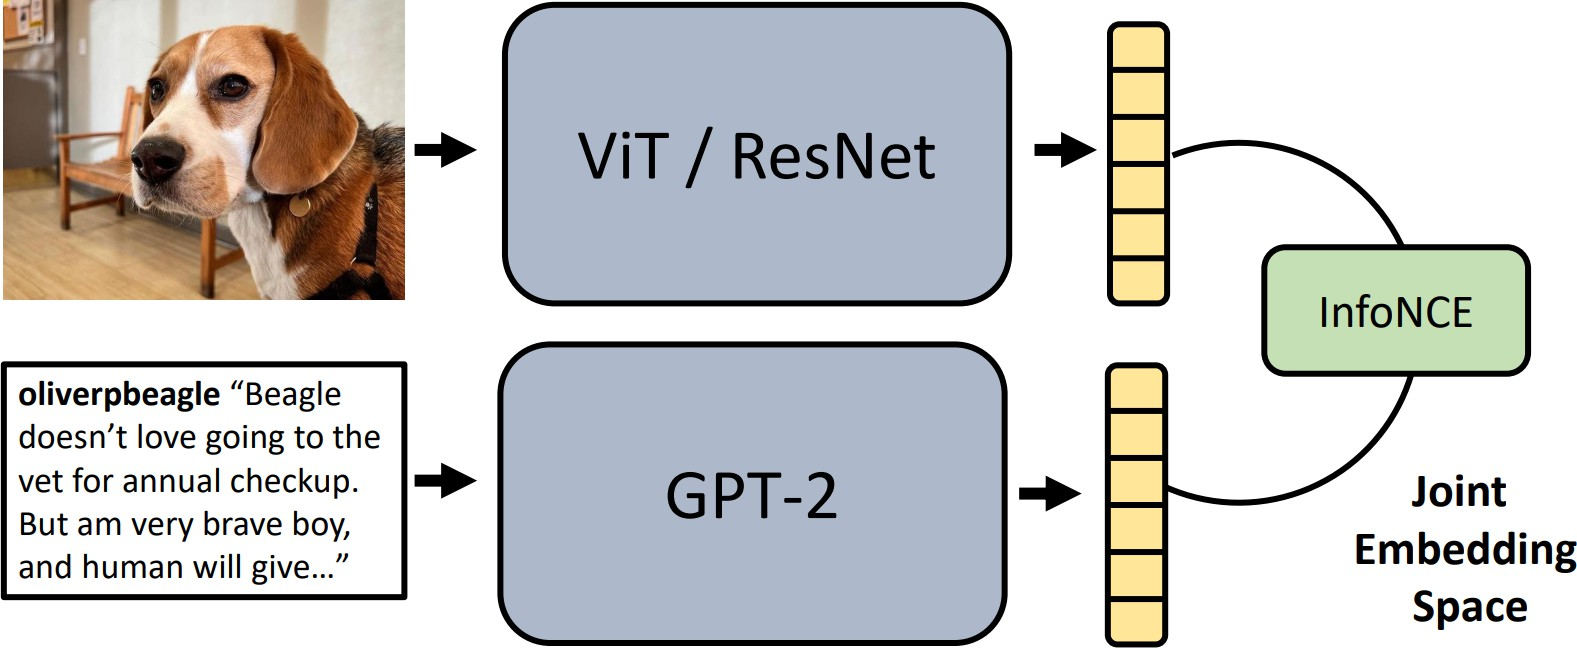
\includegraphics[width=1\textwidth,height=0.6\textheight,keepaspectratio]{images/video/slide_51_1_img.jpg}
    \end{figure}
    \footnotesize{[Radford et al., Learning Transferable Visual Models From Natural Language Supervision, ICML 2021]}
\framebreak
    \begin{figure}
        \centering
        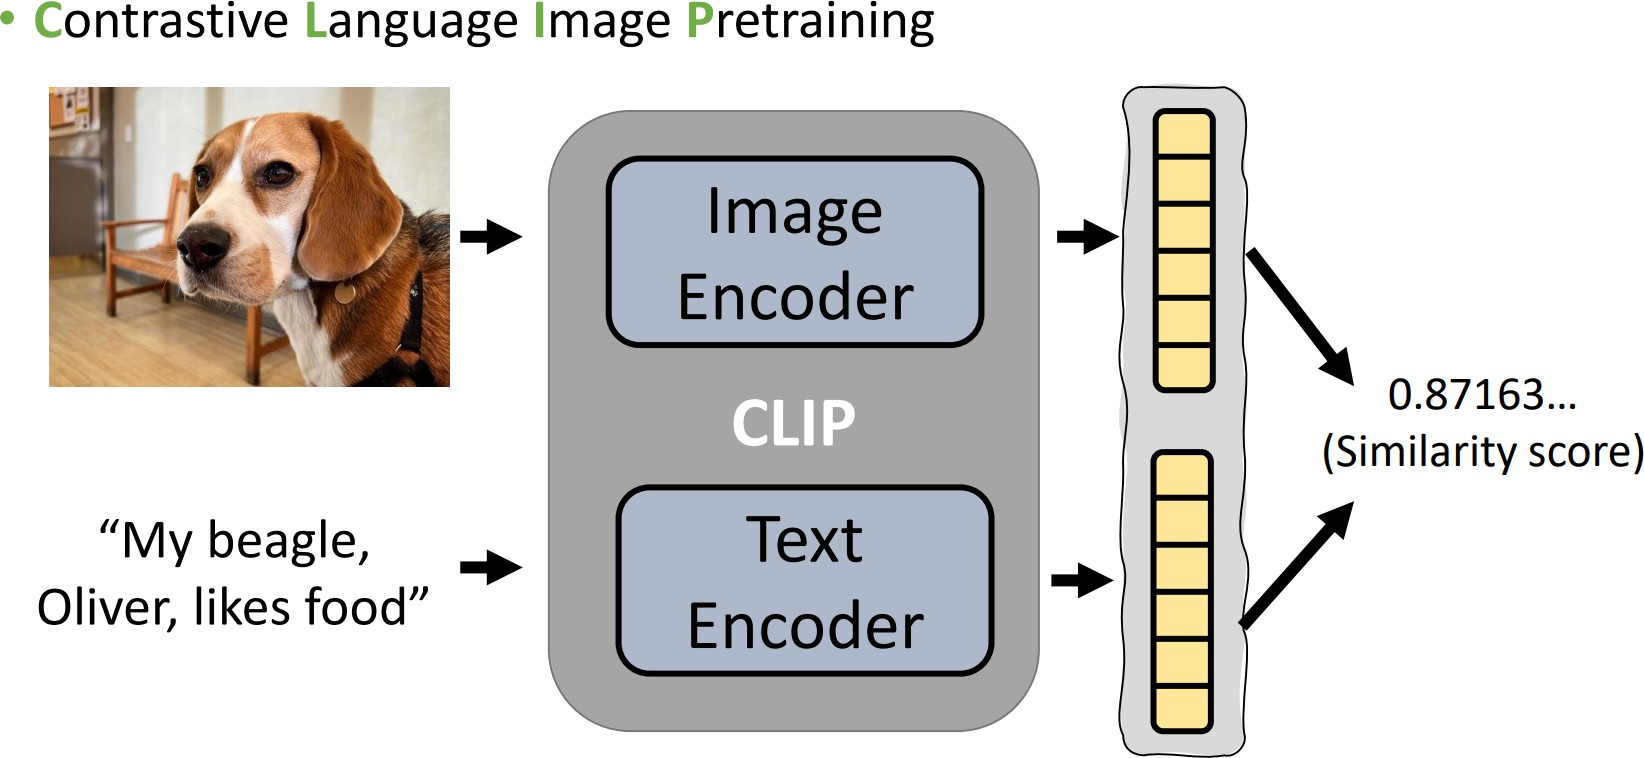
\includegraphics[width=1\textwidth,height=0.9\textheight,keepaspectratio]{images/video/slide_52_1_img.jpg}
    \end{figure}
\framebreak
    \begin{figure}
        \centering
        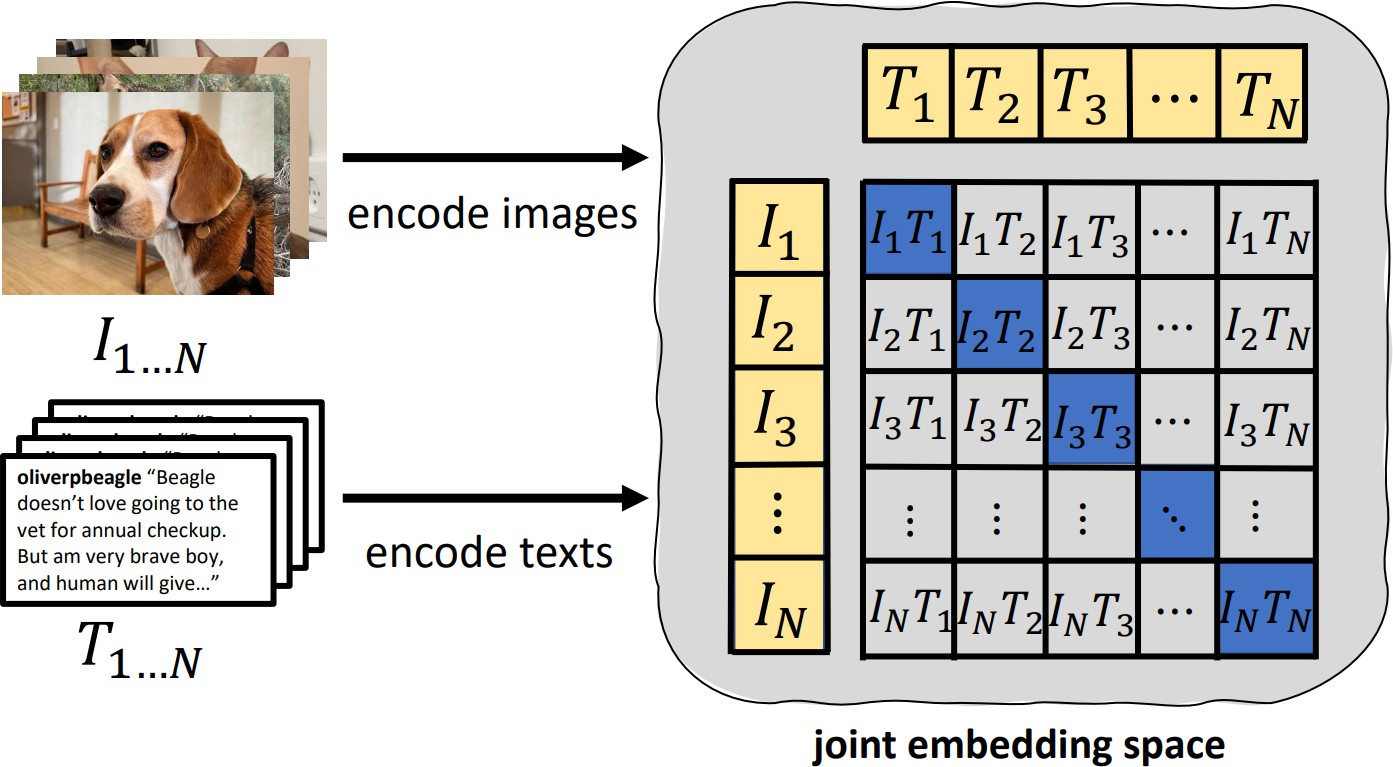
\includegraphics[width=1\textwidth,height=0.9\textheight,keepaspectratio]{images/video/slide_53_1_img.jpg}
    \end{figure}
\framebreak
    \begin{figure}
        \centering
        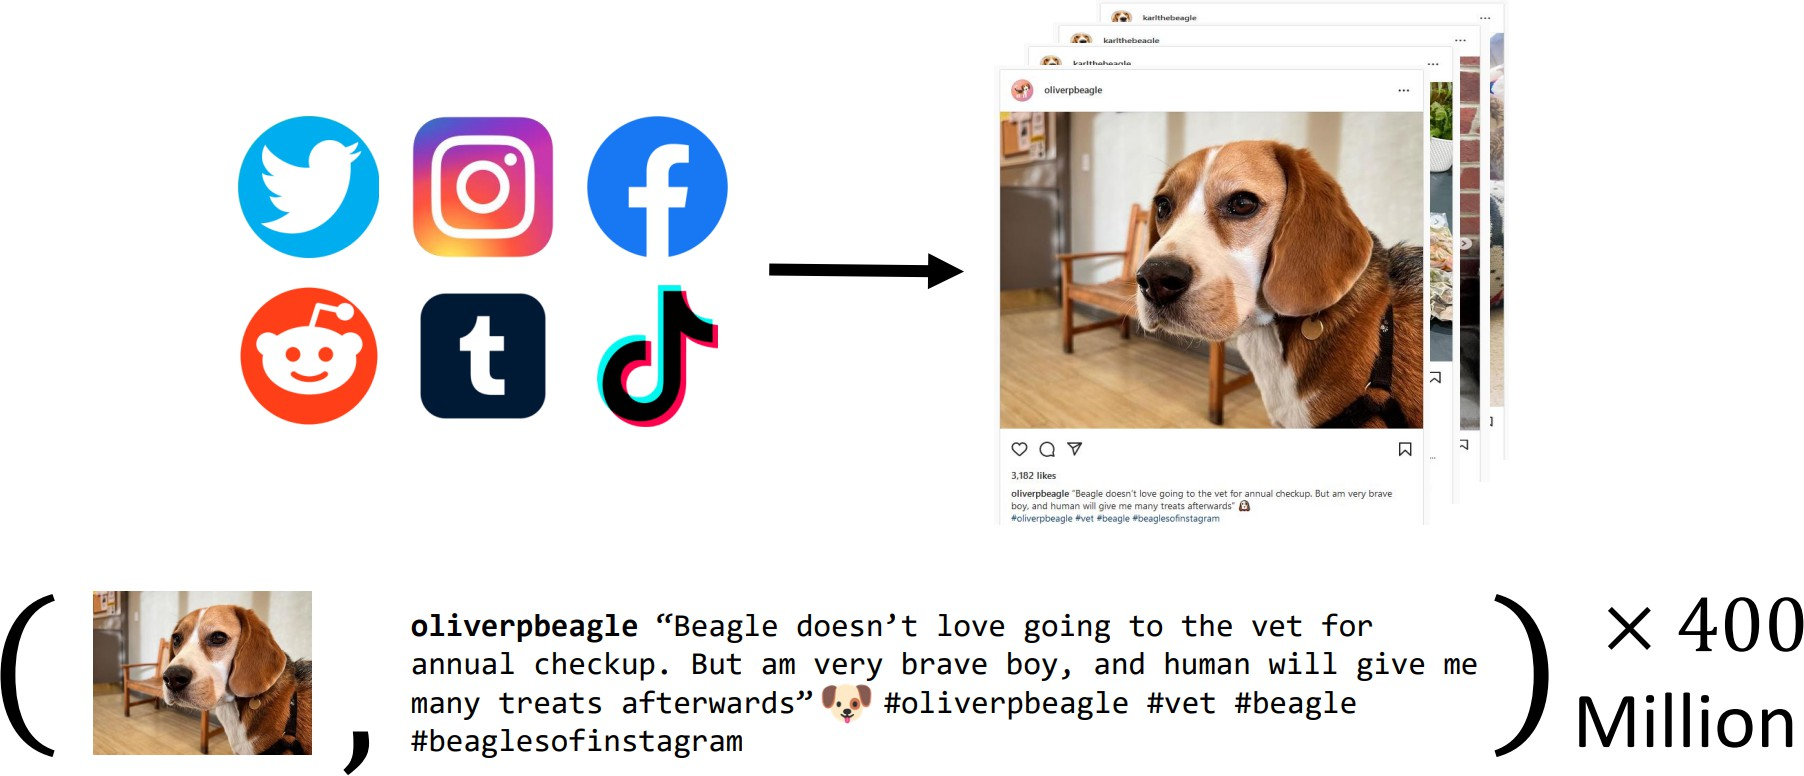
\includegraphics[width=1\textwidth,height=0.9\textheight,keepaspectratio]{images/video/slide_54_1_img.jpg}
    \end{figure}
\end{frame}


\subsection{CLIP – Zero Shot Capabilities}
\begin{frame}[allowframebreaks]{CLIP – Zero Shot Capabilities}
    \textbf{Zero-Shot Learning with CLIP:} CLIP can classify images into categories without any task-specific training by leveraging the learned image-text embeddings.

    \begin{itemize}
        \item \textbf{How it Works:} For a given image, CLIP computes its embedding and compares it with the embeddings of text descriptions of potential classes.
        \item \textbf{Similarity Measure:} The class with the highest similarity score is selected as the predicted label.
        \item \textbf{Advantages:} This approach allows CLIP to generalize to new tasks and categories without requiring additional training data.
    \end{itemize}
\framebreak
    \textbf{Example:} CLIP can classify an image of a dog as "dog" by matching its embedding to text embeddings like "dog" or "cat" and picking the closest match.
    \begin{figure}
        \centering
        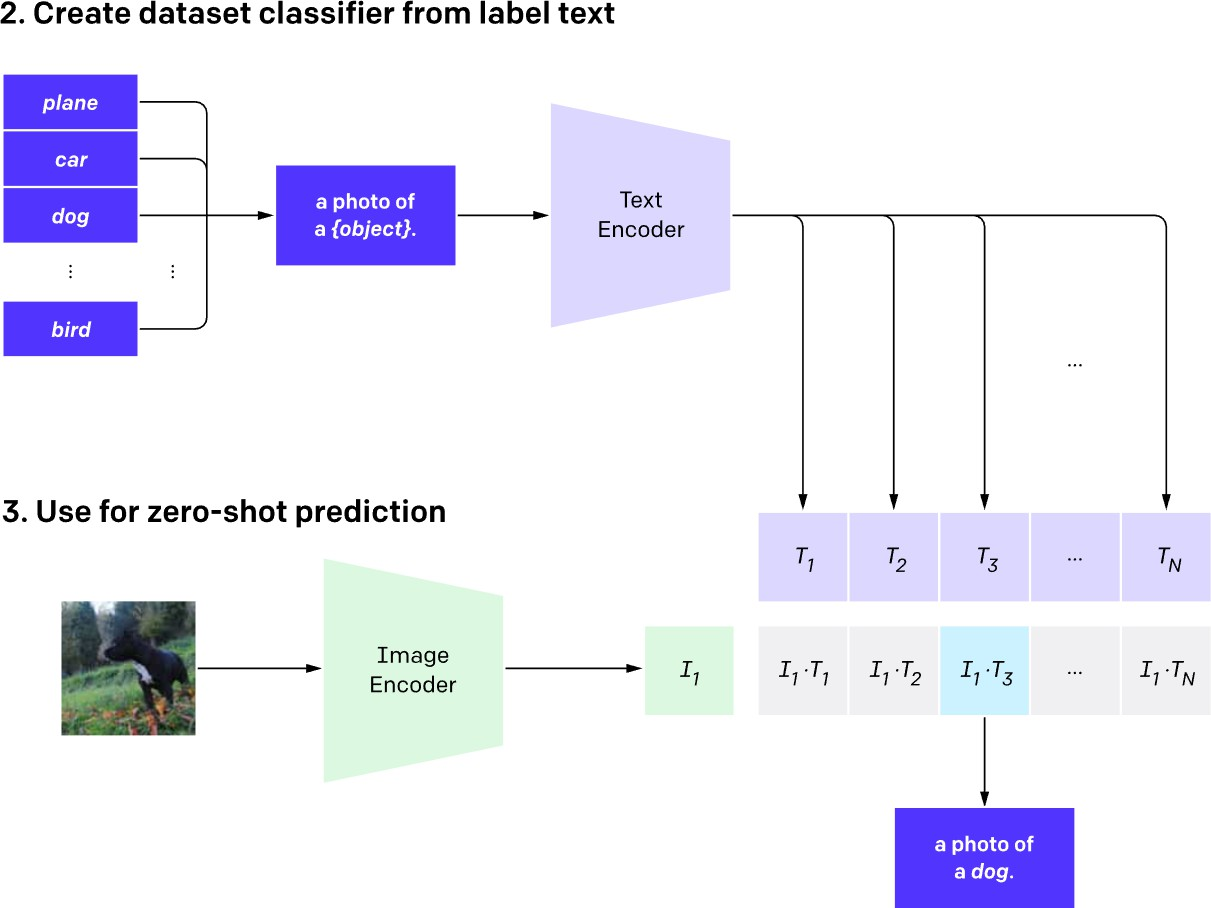
\includegraphics[width=1\textwidth,height=0.7\textheight,keepaspectratio]{images/video/slide_55_1_img.jpg}
    \end{figure}
    % \footnotesize{\url{https://openai.com/research/clip}}
\framebreak
    \begin{figure}
        \centering
        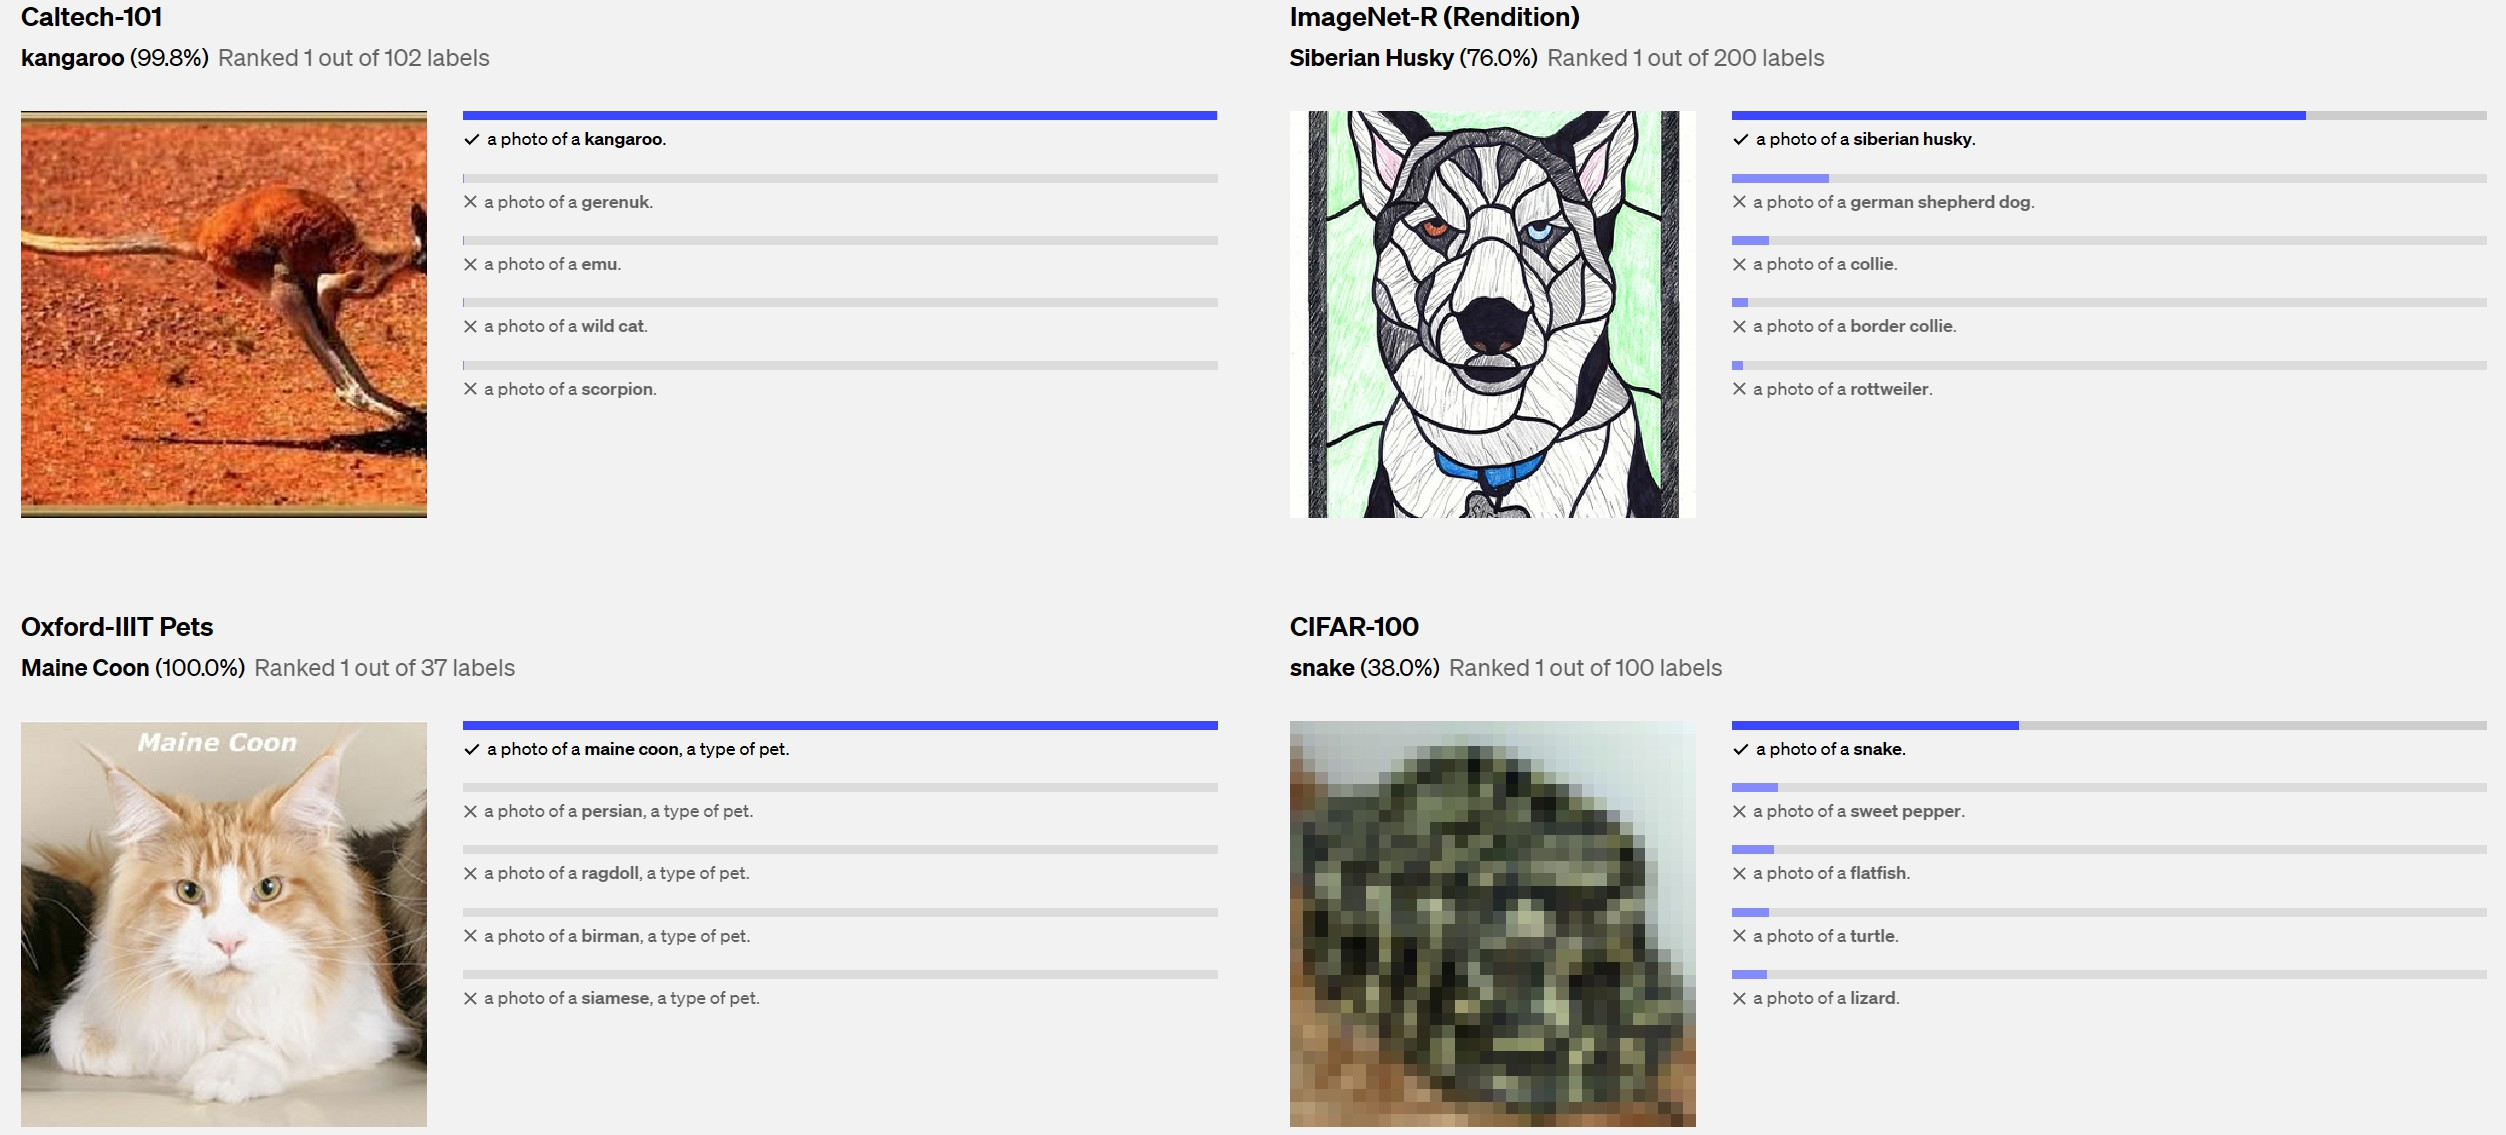
\includegraphics[width=1\textwidth,height=0.9\textheight,keepaspectratio]{images/video/slide_56_1_img.jpg}
    \end{figure}
\framebreak
    \begin{figure}
        \centering
        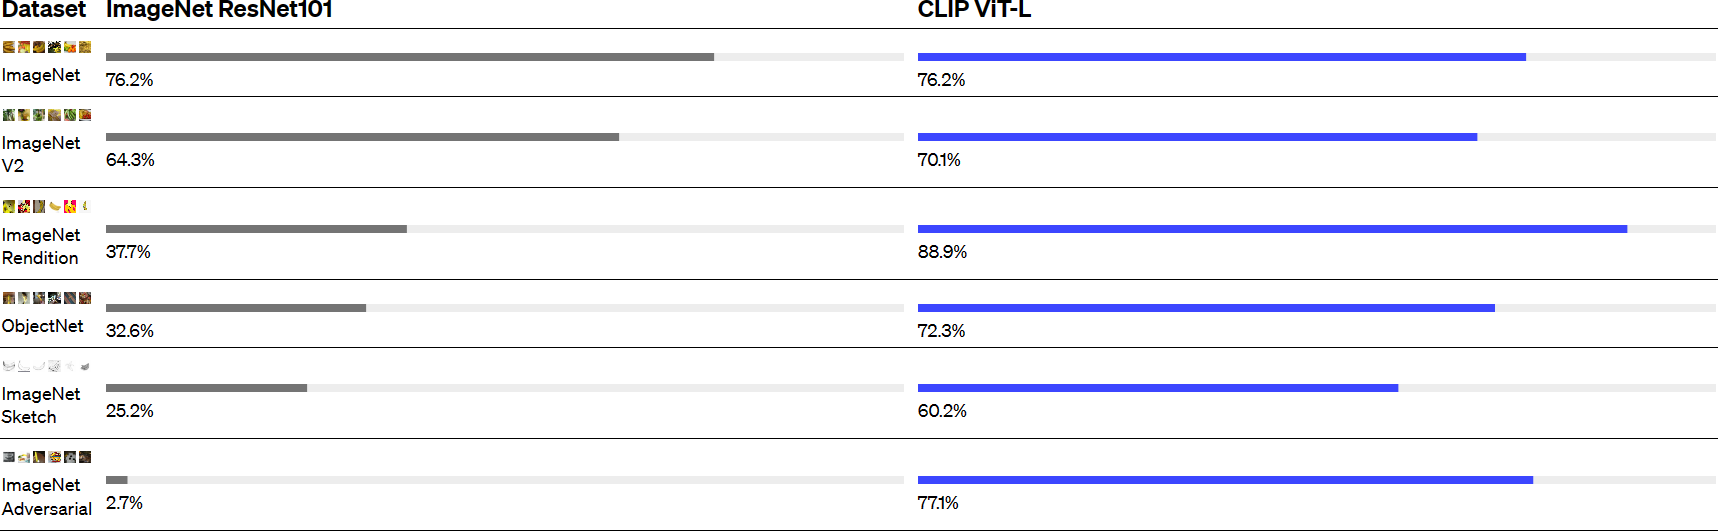
\includegraphics[width=1\textwidth,height=0.9\textheight,keepaspectratio]{images/video/slide_57_1_img.png}
    \end{figure}
\end{frame}


\subsection{Using CLIP for generative tasks}
\begin{frame}[allowframebreaks]{Using CLIP for generative tasks}
    \textbf{CLIP for Generative Tasks:} CLIP can be used to guide generative models, such as GANs or diffusion models, by providing a text-based conditioning signal.

    \begin{itemize}
        \item \textbf{Text Conditioning:} The text encoder of CLIP can be used to condition the generative model on specific text prompts, allowing it to generate images that match the given descriptions.
        \item \textbf{Loss Function:} The similarity between generated image embeddings and text embeddings can be used as a loss function to optimize the generative model.
        \item \textbf{Applications:} This approach is useful for tasks like text-to-image synthesis, where the goal is to generate images based on textual descriptions.
    \end{itemize}
\framebreak
    \begin{figure}
        \centering
        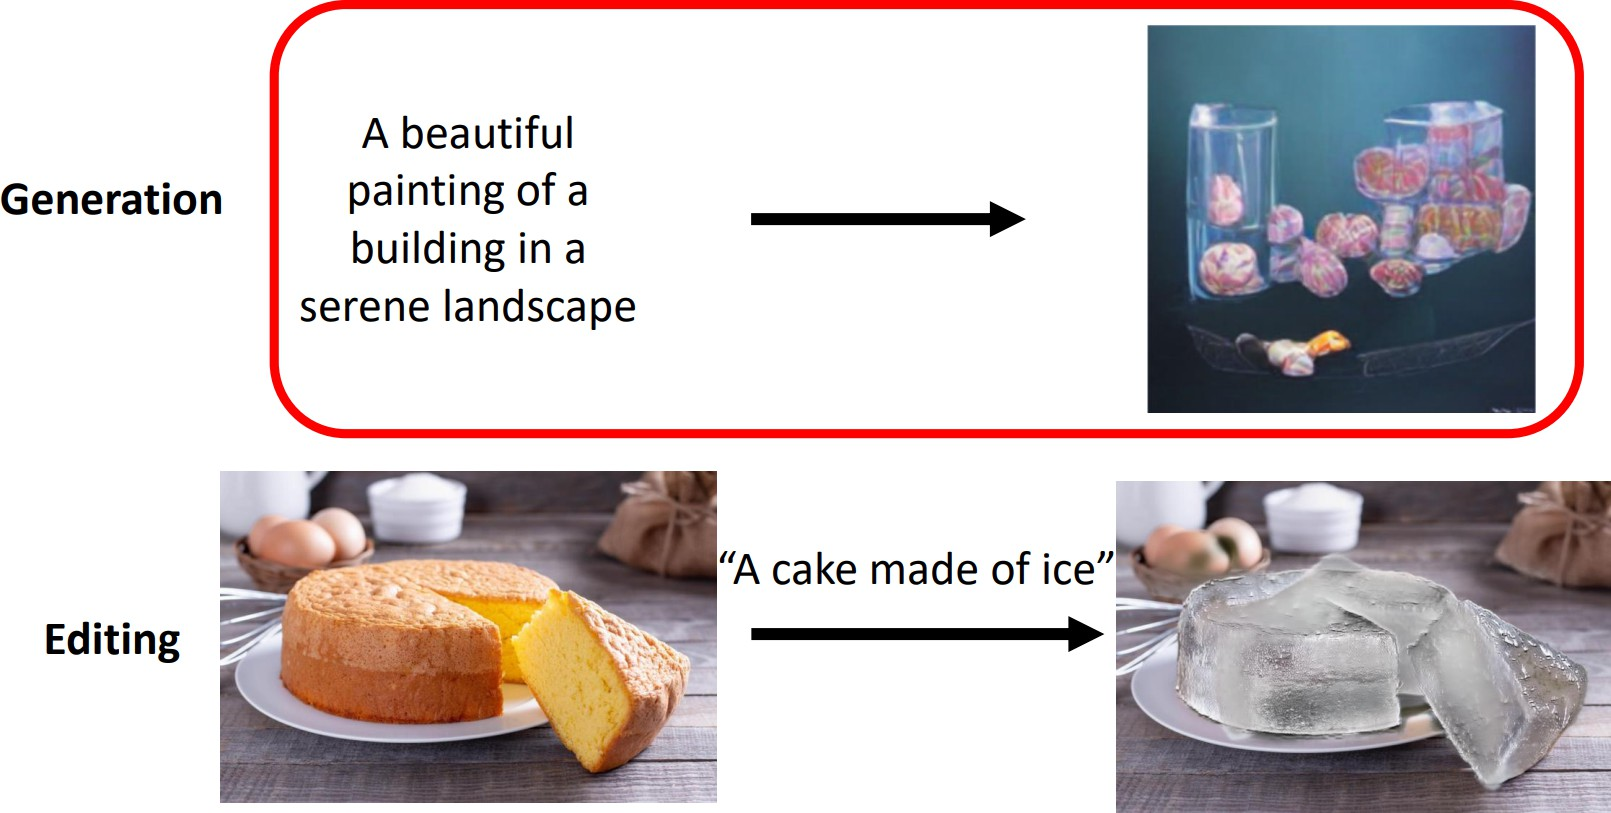
\includegraphics[width=1\textwidth,height=0.9\textheight,keepaspectratio]{images/video/slide_58_1_img.jpg}
    \end{figure}
\end{frame}